\documentclass{article}

%Paquetes AMS
\usepackage{amsmath}
\usepackage{amsfonts}
\usepackage{amssymb}

%Fuente de letra
\usepackage{utopia}

%Márgenes y demás
\usepackage{vmargin}
\usepackage{parskip}
\usepackage{setspace}
\usepackage{tcolorbox}

% Gráficas y demás
\usepackage{pgfplots}
\usepackage{graphicx}

%CUERPO
\begin{document}
	
	
	
	%%%%%%%%%%%%%%%% EJERCICIO 1 %%%%%%%%%%%%%%%%
	\section{Problema 1}
	\color{blue}
	El n{\'u}mero de hijos de las familias de una determinada
	barriada de una ciudad es una variable estad{\'\i}stica de la que se
	conocen los siguientes datos:
	
	\hskip 3cm $\begin{array}{|c|c|c|c|}
	x_{i} & n_{i} & N_{i} & f_{i}
	\\   \hline
	0 & 80  &     & 0\mbox{.}16 \\
	1 & 110 &     &      \\
	2 &     & 320 &      \\
	3 &     &     & 0\mbox{.}18 \\
	4 & 40  &     &      \\
	5 &     &     &      \\
	6 & 20  &     &  \\ \hline
	\end{array}$   \hskip 1.5cm $\begin{array}{l}  n_i: \ \mbox{frecuencias absolutas} \\ N_i:  \ \mbox{frecuencias absolutas acumuladas}\\ f_i:  \ \mbox{frecuencias relativas}\end{array}$
	\begin{enumerate}
		\item Completar la tabla de frecuencias.
		\item Representar la distribuci{\'o}n mediante un diagrama de
		barras y la curva de distribuci{\'o}n.
		\item Promediar los valores de la variable mediante diferentes
		medidas. Interpretarlas. \\
		%    \item Calcular los valores mediano y modal. Interpretarlos.
	\end{enumerate}
	
	\color{black}
	\problem
Se han lanzado dos dados varias veces, obteniendo los resultados que se presentan en la siguiente tabla, donde $X$ designa el resultado del primer dado  e $Y$ el resultado del segundo:
$$
   \begin{array}{|c|c|c|c|c|c|c|c|c|c|c|c|c|c|c|c|c|c|c|c|c|c|c|c|c|}
 X & 1 & 2 & 2 & 3 & 5 & 4 & 1 & 3 & 3 & 4 & 1 & 2 & 5 & 4 & 3 & 4 & 4 & 5 & 3 & 1 & 6 & 5 & 4 & 6 \\ \hline
 Y & 2 & 3 & 1 & 4 & 3 & 2 & 6 & 4 & 1 & 6 & 6 & 5 & 1 & 2 & 5 & 1 & 1 & 2 & 6 & 6 & 2 & 1 & 2 & 5 \\
   \end{array}
$$

  \begin{enumerate}
     \item Construir la tabla de frecuencias.
     \item Calcular las puntuaciones medias obtenidas con cada dado y ver cuales son m\'as homog\'eneas.
     \item ?`Qu\'e
      resultado del segundo dado es  m\'as frecuente cuando en el primero se obtiene
        un 3?
     \item Calcular la puntuaci\'on m\'axima del 50\% de las puntuaciones m\'as bajas obtenidas con el primer dado si con el segundo se ha obtenido un 2 o un 5.
   \end{enumerate}

Antes de resolver el ejercicio crearemos un nuevo enunciado, pues no tiene sentido calcular las cosas que nos piden, cuando estas dependen de la aleatoriedad. En nuestro nuevo enunciado, la variable X será el número de personas que componen distintas familias de Granada, y la variable Y es el número de habitaciones que tienen en sus casas. Resolvemos ahora el ejercicio.

\subproblem
Calculamos la tabla de frecuencia y además, los elementos que necesitaremos durante el ejercicio.

\begin{table}[h]
    \centering
    \begin{tabular}{|c|c|c|c|c|}
        \hline
         $x_i$ & $n_{i.}$ & $x_{i}n_{i.}$ & $x_i^2 n_{i.}$ \\ \hline
         1 & 4 & 4 & 4 \\ \hline 
         2 & 3 & 6 & 12 \\ \hline 
         3 & 5 & 15 & 45\\ \hline 
         4 & 6 & 24 & 96 \\ \hline 
         5 & 4 & 20 & 100 \\ \hline 
         6 & 2 & 12 & 72 \\ \hline 
          & 24 & 81 & 329 \\ \hline 
    \end{tabular}
\end{table}

\begin{table}[h]
    \centering
    \begin{tabular}{|c|c|c|c|}
        \hline
         $y_j$ & $n_{.j}$ & $y_{j}n_{.j}$ & $y_{j}^2n_{.j}$ \\ \hline
         1 & 6 & 6 & 6 \\ \hline 
         2 & 6 & 12 & 24 \\ \hline 
         3 & 2 & 6 & 18 \\ \hline 
         4 & 2 & 8 & 32 \\ \hline 
         5 & 3 & 15 & 75 \\ \hline 
         6 & 5 & 30 & 180 \\ \hline
           & 24 & 77 & 335 \\ \hline 
    \end{tabular}
\end{table}

\subproblem
Calculamos la media de nuestras variables:

\begin{equation*}
    \overline{x} = \dfrac{1}{n} \sum_{i=1}^k x_i n_{i.} = \dfrac{81}{24} = 3.375 \approx 3 hijos
    \hspace{1cm}
    \overline{y} = \dfrac{1}{n} \sum_{k=1}^p y_j n_{j.} = \dfrac{77}{24} = 3.2083 \approx 3 habitaciones
\end{equation*}

Ahora calculamos la desviación típica de cada variable para poder calcular el coeficiente de variación de Pearson y ver cuál es más homogénea:

\begin{equation*}
    \sigma_{x} = \sqrt{\dfrac{328}{24}-3.375^2} = 1.5224 hijos
    \hspace{1cm}
    \sigma_{y} = \sqrt{\dfrac{335}{24}-3.2083^2} = 1.9144 habitaciones
\end{equation*}

\begin{equation*}
    CV_{x} = \dfrac{\sigma_x}{\overline{x}} = 0.4511
    \hspace{1cm}
    CV_{y} = \dfrac{\sigma_y}{\overline{y}} = 0.5967
\end{equation*}

Como vemos, los resultados de la primera variable son más homogéneos pues su coeficiente de variación de Pearson es menor.

\subproblem
Mirando la tabla de resultados, vemos que cuando las familias tenían 3 habitaciones en sus casas, el número de hijos más frecuente es el 4, con 2 veces, luego $M_0=4$.

\subproblem
Vamos a calcular la media de $X/Y$ cuando las familias tienen dos o cinco habitaciones en sus casa. Mirando la tabla de resultados obtenemos:

\begin{table}[ht]
    \begin{tabular}{|c|c|c|}
        \hline
         $x_i/Y$ & $n_{i}$ & $N_{i}$ \\ \hline
         1 & 1 & 1 \\ \hline 
         2 & 1 & 2 \\ \hline 
         3 & 1 & 3 \\ \hline 
         4 & 3 & 6 \\ \hline 
         5 & 1 & 7 \\ \hline  
         6 & 2 & 9 \\ \hline 
    \end{tabular}
\end{table}

Como $n/2 = 4.5$ y la frecuencia absoluta acumulada inmediatamente superior a este número es $N_{4} = 6$, deducimos que la mediana es $M_e = 4$.

	
	
	
	%%%%%%%%%%%%%%%% EJERCICIO 2 %%%%%%%%%%%%%%%%
	\section{Problema 2}
	\color{blue}
	La puntuaci{\'o}n obtenida por 50 personas que se presentaron a  una  prueba
	de selecci{\'o}n, sumadas las puntuaciones de los distintos tests, fueron:
	
	\smallskip
	\centerline{$174,185,166,176,145,166,191,175,158,156,156,187,162,172,197,181,151,$}
	\smallskip
	\centerline{$161,183,172,162,147,178,176,141,170,171,158,184,173,169,162,172,181,$}
	\smallskip
	\centerline{$187,177,164,171,193,183,173,179,188,179,167,178,180,168,148,173.$}
	\vskip -1cm
	\begin{enumerate}
		\item Agrupar los datos en intervalos de amplitud 5 desde 140 a 200 y dar la tabla de frecuencias.
		\item Representar la distribuci{\'o}n mediante un histograma, poligonal de
		frecuencias y curva de distribuci{\'o}n. \\
	\end{enumerate}
	
	\color{black}
	    POBLACIÓN: Las personas que se presentaron a la prueba de selección\\
    TAMAÑO: 50\\
    MODALIDADES: Los intervalos que contienen las notas que han obtenido las personas en la prueba
    
    \vspace{5mm}
    \subproblem
    Agrupar los datos en intervalos de amplitud 5 desde 140 a 200 y dar la tabla de frecuencias.
    \\
    \begin{center}
    \begin{tabular}{| c | c | c | c | c |}
        \hline
        $x_i$ & $n_i$ & $N_i$ & $f_i$ & $F_i$ \\ \hline
        (140-145] & 2 & 2 & 0,04 & 0,04 \\
        (145-150] & 2 & 4 & 0,04 & 0,08 \\
        (150-155] & 1 & 5 & 0,02 & 0,1 \\
        (155-160] & 4 & 9 & 0,08 & 0,18 \\
        (160-165] & 5 & 14 & 0,1 & 0,28 \\
        (165-170] & 6 & 20 & 0,12 & 0,4 \\
        (170-175] & 10 & 30 & 0,2 & 0,6 \\
        (175-180] & 8 & 38 & 0,16 & 0,76 \\
        (180-185] & 6 & 44 & 0,12 & 0,88 \\
        (185-190] & 3 & 47 & 0,06 & 0,94 \\
        (190-195] & 2 & 49 & 0,04 & 0,98 \\
        (195-200] & 1 & 50 & 0,02 & 1 \\
        \hline
    \end{tabular} 
    \end{center}
    
    \vspace{5mm}
    
    Establecemos los intervalos de amplitud 5, empezando con 140 y terminando con 200. Para cada intervalo, contamos cuantas personas han obtenido una puntuación que esté dentro de dicho intervalo. Estas son las frecuencias absolutas ($n_i$). 
    Para la frecuencia absoluta acumulada ($N_i$), sumamos la frecuencia absoluta de la modalidad que estamos analizando a la frecuencia absoluta acumulada de la modalidad anterior. O lo que es lo mismo, sumamos las frecuencias absolutas de todas las modalidades hasta la que estamos analizando: $N_i=n_1 + n_2 + ... + n_i$. 
    Para frecuencia relativa, dividimos cada $n_i$ entre n, es decir, entre el número total de individuos de la población, la frecuencia absoluta acumulada de la última modalidad. 
    Para la frecuencia relativa acumulada hacemos lo mismo que para la absoluta acumulada pero con la frecuencia relativa: sumamos las frecuencias relativas de todas las modalidades hasta la que estamos analizando: $F_i=f_1 + f_2 + ... + f_i$. 
    
    \vspace{10mm}
    \subproblem
    Representar la distribución mediante un histograma, poligonal de frecuencias y curva de distribución.
    
    \begin{center}
    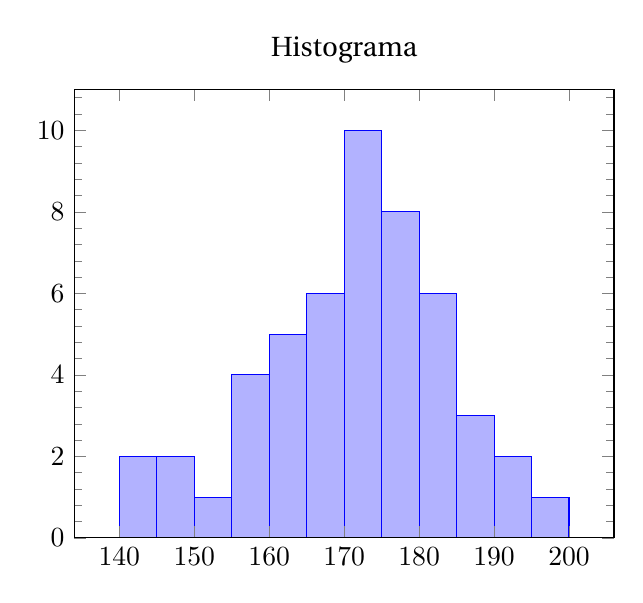
\begin{tikzpicture}
        \begin{axis}[
            title={Histograma},
            ymin=0, ymax=11,
            minor y tick num = 4,
            area style,
            ]
        \addplot+[ybar interval,mark=no] plot coordinates { (140, 2) (145, 2) (150, 1) (155, 4) (160, 5) (165, 6) (170, 10) (175, 8) (180, 6) (185, 3) (190, 2) (195, 1) (200, 0) };
        \end{axis}
    \end{tikzpicture}
    \end{center}
    
    Para el histograma, en el eje X tenemos las modalidades ($x_i$) y en el eje Y un múltiplo de $h_{i}$ ($h_{i}=\frac{fi}{a}$). En este caso, las amplitudes de todos los intervalos son iguales: 5. 
    
    \vspace{5mm}
    \begin{center}
    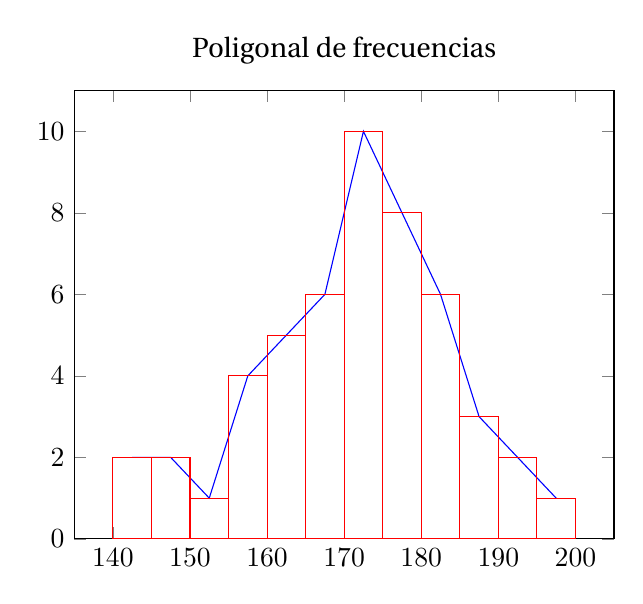
\begin{tikzpicture}
    \begin{axis}[
        title={Poligonal de frecuencias},
        xmin=135, xmax=205,
        ymin=0, ymax=11,
        xtick={140,150,160,170,180,190,200},
        ytick={0,2,4,6,8,10},
        legend pos=north west,
        ymajorgrids=false,
        grid style=dashed,
    ]

    \addplot[
        color=blue,
        ]
        coordinates {
        (142.5,2)(147.5,2)(152.5,1)(157.5,4)(162.5,5)(167.5,6)(172.5,10)(177.5,8)(182.5,6)(187.5,3)(192.5,2)(197.5,1)
        };
            [
            ymin=0, ymax=11,
            minor y tick num = 4,
            area style,
            ]
        \addplot+[ybar interval,mark=no] plot coordinates { (140, 2) (145, 2) (150, 1) (155, 4) (160, 5) (165, 6) (170, 10) (175, 8) (180, 6) (185, 3) (190, 2) (195, 1) (200, 0) };
    
    \end{axis}
    \end{tikzpicture}
    \end{center}
    
    Para el poligonal de frecuencias, los ejes son los mismos que para el histograma. En este caso, unimos los puntos que corresponden a las marcas de clase de los intervalos en el histograma. Para hallar dichas marcas de los intervalos, aplicamos la siguiente expresión: $c_i=\frac{e_{i-1}+e_i}{2}$.
    
    \begin{center}
    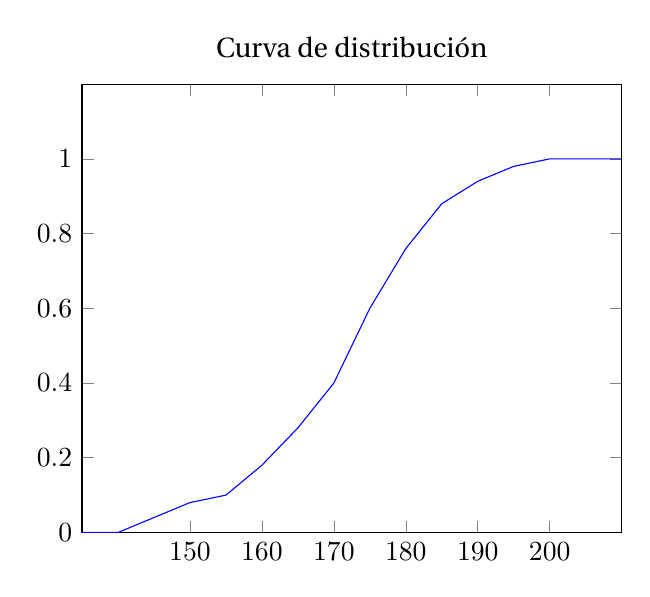
\begin{tikzpicture}
    \begin{axis}[
        title={Curva de distribución},
        xmin=135, xmax=210,
        ymin=0, ymax=1.2,
        xtick={150,160,170,180,190,200},
        ytick={0,0.2,0.4,0.6,0.8,1},
        legend pos=north west,
        ymajorgrids=false,
        grid style=dashed,
    ]

    \addplot[
        color=blue,
        ]
        coordinates {
        (135,0)(140,0)(145,0.04)(150,0.08)(155,0.1)(160,0.18)(165,0.28)(170,0.4)(175,0.6)(180,0.76)(185,0.88)(190,0.94)(195,0.98)(200,1)(205,1)(210,1)
        };
    
    \end{axis}
    \end{tikzpicture}
    \end{center}
    
    En la curva de distribución, en el eje X tenemos los extremos superiores de los intervalos $(e_i)$ y en el eje Y, $F(e_i)$. Pintamos la curva que une los puntos tal que $F(e_i)=\displaystyle\sum_{j=1}^{i}f_{j}=F_i$. En este caso tenemos que la curva es continua. $F(e_i)$ es 0 para valores menores que $e_1$ y 1 para valores mayores que el último intervalo $e_k$.
	
	
	
	%%%%%%%%%%%%%%%% EJERCICIO 3 %%%%%%%%%%%%%%%%
	\section{Problema 3}
	\color{blue}
	La distribuci{\'o}n de la renta familiar  en el a{\~n}o 2003 por comunidades aut{\'o}nomas se recoge en la
	siguiente tabla:
	
	$\begin{array}{|r|c|c|c|c|c|c|c|}
	\multicolumn{1}{c|}{I_{i}} & n_{i} & N_{i} & f_{i} & F_{i} & c_{i} & a_{i} & h_{i} \\
	\hline
	(8300,9300] & 2 &  &  &  &  &  &  \\
	,10200] &  & 5 &  &  &  &  &  \\
	&  &  &  & 10/18 &  & 1100 &  \\
	&  &  & 2/18 &  & 12000 &  &  \\
	& 4 &  &  &  &  &  & 0\mbox{.}005/18 \\
	&  & 18 &  &  &  &  & 0\mbox{.}002/18 \\  \hline
	\end{array}$ \hskip 1cm $\begin{array}{l}  n_i: \ \mbox{frecuencias absolutas} \\ N_i:  \ \mbox{frec. absolutas acumuladas}\\ f_i:  \ \mbox{frecuencias relativas}
	\\ F_i:  \ \mbox{frec. relativas acumuladas}\\ c_i:  \ \mbox{marcas de clase}\\ a_i:  \ \mbox{amplitudes} \\ h_i:  \ \mbox{densidades de frecuencia}\end{array}$
	\begin{enumerate}
		\item Completar la tabla.
		\item Representar la distribuci{\'o}n mediante un histograma,
		poligonal de frecuencias y curva de distribuci{\'o}n.
		\item ?`Cu{\'a}ntas comunidades presentan una renta menor o igual
		que 12700 euros? ?`Y cu{\'a}ntas superior a 11300 euros? \\
	\end{enumerate}
	
	\color{black}
	\problem
Se sacan dos bolas sucesivamente sin devolución de una urna que contiene 3 bolas rojas distinguibles y 2 blancas distinguibles. \\ \\

\subproblem
Describir el espacio de probabilidad asociado a este experimento. \\
$\omega = ${(R1,R2), (R1,R3), (R1,B1), (R1,B2), (R2,R1), (R2,R3), (R2,B1), (R2,B2), (R3,R1), (R3,R2), (R3,B1), (R3,B2), (B1,R1), (B1,R2), (B1,R3), (B1,B2), (B2,R1), (B2,R2), (B2,R3), (B2,B1)} \\ \\

\subproblem
Descomponer en sucesos elementales los sucesos: "la primera bola es roja", "la segunda bola es blanca" y calcular la probabilidad de cada uno de ellos. \\
A = La primera bola es roja: {(R1,R2), (R1,R3), (R1,B1), (R1,B2), (R2,R1), (R2,R3), (R2,B1), (R2,B2), (R3,R1), (R3,R2), (R3,B1), (R3,B2)} \\
$P(A) = \frac{12}{20} = 0'6$ \\
B = La segunda bola es blanca: {(R1,B1), (R1,B2), (R2,B1), (R2,B2), (R3,B1), (R3,B2), (B1,B2), (B2,B1)} \\
$P(B) = \frac{8}{20} = 0,4$ \\ \\

\subproblem
¿Cuál es la probabilidad de que ocurra alguno de los sucesos considerados en el apartado anterior? \\
$P(A\cup B) = P(A)+P(B)-P(A\cap B) = 0'6 + 0'4 - 0'3 = 0'7$ \\ \\

	
	
	
	%%%%%%%%%%%%%%%% EJERCICIO 4 %%%%%%%%%%%%%%%%
	\section{Problema 4}
	\color{blue}
	En una determinada empresa se realiza un estudio sobre la calidad de su
	producci{\'o}n. La distribuci{\'o}n siguiente informa sobre el n{\'u}mero de  piezas
	defectuosas encontradas en 100 cajas examinadas con 50 unidades cada una
	de ellas:
	$$\setlength{\arraycolsep}{10pt}
	\begin{array}{|c||c|c|c|c|c|c|c|c|c|c|c|} \hline
	\mbox{N${}^{\underline{o}}$ piezas defectuosas} & 0 & 1 & 2  & 3
	& 4  & 5  & 6  & 7 & 8 & 9 & 10 \\ \hline
	\mbox{N${}^{\underline{o}}$ de cajas}           & 6 & 9 & 10 & 11
	& 14 & 16 & 16 & 9 & 4 & 3 & 2 \\ \hline
	\end{array}
	$$
	
	\begin{enumerate}
		\item Calcular el n{\'u}mero medio de piezas defectuosas por caja.
		\item ?`Cuantas piezas defectuosas se encuentran m{\'a}s frecuentemente en las
		cajas examinadas?
		\item ?`Cu{\'a}l es el n{\'u}mero mediano de piezas defectuosas por caja?
		\item Calcular los cuartiles de la distribuci{\'o}n. Interpretarlos.
		\item Calcular los deciles de orden 3 y 7. Interpretarlos.
		\item Cuantificar la dispersi{\'o}n de la  distribuci{\'o}n utilizando diferentes
		medidas, interpretando los resultados  y se{\~n}alando las ventajas e
		inconvenientes de cada una. \\
	\end{enumerate}
	\color{black}
	\problem
Sea $X$ una variable aleatoria con funci{\'o}n de densidad
$$
f(x) = \left \{
\begin{array}{lc}
k_{1} (x+1) & 0 \leq x \leq 4 \\
\\ k_{2} x^{2} & 4 <x \leq 6
\end{array}
\right.
$$
Sabiendo que  $P(0 \leq X \leq 4) = 2/3$,  determinar $k_{1},\ k_{2}$, y
deducir su funci{\'o}n de distribuci{\'o}n.

Nótese que la variable aleatoria es continua y toma valores entre 0 y 6. En el desarrollo de este ejercicio, se presupondrá que la función de masa dada es correcta. 

En primer lugar, calculemos la función de distribución de la variable aleatoria. Aplicamos la siguiente expresión: $F(x) = \int_{-\infty}^x f(t) dt$. 

Si $0 \leq x \leq 4$, tenemos que: 

$$F(x) = \int_{-\infty}^x f(t) dt = \int_{-\infty}^0 0 dt + \int_0^x k_1(t+1)dt = k_1(\frac{·x^2}{2} + x)$$ 

Si $4 < x \leq 6$, tenemos que:

\begin{equation*}
\begin{split}
F(x) & = \int_{-\infty}^x f(t) dt = \int_{-\infty}^0 0 dt + \int_0^4 k_1(t+1)dt + \int_4^x k_2·t^2 dt \\
& = k_1(\frac{4^2}{2} + 4) + k_2(\frac{x^3}{3} - \frac{4^3}{3}) 
\end{split}
\end{equation*}

Sabemos que $P(0\leq X \leq 4) = F(4) - F(0^-)$. Como la variable es continua, tenemos que $F(0^-) = F(0)$. Deducimos entonces que: 

$$P(0 \leq X \leq 4) = F(4) - F(0^-) = F(4) - F(0) = k_1(\frac{4^2}{2} + 4) = 2/3 \Rightarrow k_1 = \frac{1}{18}$$

Por otra parte, para que se verifique que se trate, en efecto, de una función de distribución, se ha de verificar que: 

$$F(+\infty) = k_2(\frac{6^3}{3} - \frac{4^3}{3}) + \frac{2}{3} = 1 \Rightarrow k_2 = \frac{1}{152}$$

Por tanto, la función de distribución viene dado por la siguiente expresión: 

\begin{equation*}
	F(x) = \left \{
	\begin{array}{lcc}
	0 & x < 0 \\
	\frac{1}{18}(\frac{x^2}{2} + x) & 0 \leq x \leq 4 \\
	\frac{x^3}{456} + \frac{10}{19} & 4 <x \leq 6 \\
	1 & x > 6
	\end{array}
	\right.
\end{equation*}

	
	
	
	%%%%%%%%%%%%%%%% EJERCICIO 5 %%%%%%%%%%%%%%%%
	\section{Problema 5}
	\color{blue}
	Dadas las siguientes distribuciones:
	
	\setlength{}{4pt}
	$\begin{array}{|c|c|c|c|c|c|} \hline
	I_{i}^{(1)} & (0,1] & (1,2] & (2,3] & (3,4] & (4,5] \\ \hline
	n_{i}^{(1)} & 12  & 13  &  11 &  8  &  6  \\ \hline
	\end{array}$
	
	\setlength{}{4pt}
	$\begin{array}{|c|c|c|c|c|c|} \hline
	I_{i}^{(2)} & (0,1] & (1,3] & (3,6] & (6,10] & (10,12] \\ \hline
	n_{i}^{(2)} &  1   &  6  &  7  &  12  &  2  \\ \hline
	\end{array}$
	
	%$$\setlength{\extrarowheight}{4pt}
	% \begin{array}{|c|c|c|c|c|c|} \hline
	%    I_{i}^{(3)} & (0,1] & (1,3] & (3,4] & (4,5] & (5,7] \\ \hline
	%   n_{i}^{(3)} &  10  & 15  &  12 & 10  &  7  \\ \hline
	%\end{array}
	%$$
	
	
	
	
	
	Calcular para cada una de ellas:
	\begin{enumerate}
		\item Medias aritm{\'e}tica, arm{\'o}nica y geom{\'e}trica.
		\item El valor m{\'a}s frecuente.
		\item El valor superado por el 50 \% de las observaciones.
		\item Recorrido,   recorrido   intercuart{\'\i}lico   y   desviaci{\'o}n t{\'\i}pica.
		Interpretarlos. ?`Qu{\'e} distribuci{\'o}n es m{\'a}s homog{\'e}nea? \\
	\end{enumerate}
	\color{black}
	
\problem
Una urna contiene 5 bolas blancas y 3 rojas. Se extraen 2 bolas simultáneamente. Calcular la probabilidad de obtener: \\ \\
\subproblem
a) dos bolas rojas \\
A1 = primera roja, A2 = segunda roja \\
$P(A1 \cap A2) = \frac{3}{8} * \frac{2}{7} = 0'375*0'286 = 0'107$ \\ \\
\subproblem
b) dos bolas blancas \\ 
B1 = primera blanca, B2 = segunda roja \\
$P(B1 \cap B2) =  \frac{5}{8} * \frac{4}{7} = 0'625 * 0'571 = 0'357$ \\ \\
\subproblem
c) una blanca y otra roja \\
$P((A1 \cap B2)\cup (A2 \cap B1)) = \frac{3}{8}*\frac{5}{7} + \frac{5}{8}*\frac{3}{7} = 0'536$ \\
	
	
	
	%%%%%%%%%%%%%%%% EJERCICIO 6 %%%%%%%%%%%%%%%%
	\section{Problema 6}
	\color{blue}
	Un m{\'o}vil efect{\'u}a un recorrido de 100 km en dos sentidos. En
	uno  va a
	una velocidad constante de $V_1$=60 km/h y en el otro va a una velocidad
	constante de $V_2$=70 km/h. Calcular la velocidad media del recorrido. \\
	\newline
	\color{black}
	\problem

Se consideran dos urnas: la primera con 20 bolas, de las cuales  18 son blancas, y  la segunda con 10 bolas, de las cuales  9  son  blancas.  Se extrae una bola de la segunda urna y  se  deposita  en  la  primera; si a continuaci{\'o}n, se extrae una bola de {\'e}sta,  calcular  la  probabilidad  de que sea blanca.

Para abordar este problema, antes de hacer nada, le daremos nombre a los sucesos que queremos estudiar:

$B_{i}$ = Sacar bola blanca en la caja i.\\
$N_{i}$ = Sacar bola negra en la caja i.\\

Lo que queremos calcular es la probabilidad de $B_{1}$ teniendo en cuenta que añadimos una bola a la urna 1 de la  urna 2. Procedemos con los cálculos:

\begin{equation*}
    P(B_{1}) = P(B_{2}) \cdot P(B_{1}/B_{2}) + (N_{2}) \cdot P(B_{1}/N_{2}) = \dfrac{9}{10} \cdot \dfrac{19}{21} + \dfrac{1}{10} \cdot \dfrac{18}{21} = 0.9
\end{equation*}

	
	
	
	%%%%%%%%%%%%%%%% EJERCICIO 7 %%%%%%%%%%%%%%%%
	\section{Problema 7}
	\color{blue}
	Las acciones de una empresa han producido los  siguientes  rendimientos
	netos anuales:
	$$
	\begin{array}{cc}
	\mbox{A{\~n}o} & \mbox{Rentabilidad} \\ \hline
	1994  &        12\%     \\
	1995  &        10\%     \\
	1996  &         7\%     \\
	1997  &         6\%     \\
	1998  &         5\%     \\
	\end{array}
	$$
	Obtener el rendimiento neto medio en esos cinco a{\~n}os. \\
	\color{black}
	\problem \\

\subproblem \\

A = Sacar blanca en la primera urna

B = Sacar blanca en la segunda urna

C = Sacar blanca en la tercera urna \\


$P(Sacar\ 4 \ blancas) = P(U_1)P(A|U_1) + P(U_2)P(B|U_2) + P(U_3)P(C|U_3) = \\


\dfrac{1}{3}(\dfrac{5}{10}\cdot\dfrac{4}{9}\cdot\dfrac{3}{8}\cdot\dfrac{2}{7}) + 
  \dfrac{1}{3}(\dfrac{6}{10}\cdot\dfrac{5}{9}\cdot\dfrac{4}{8}\cdot\dfrac{3}{7}) + 
  \dfrac{1}{3}(\dfrac{7}{10}\cdot\dfrac{6}{9}\cdot\dfrac{5}{8}\cdot\dfrac{4}{7}) = 0.0873$ \\

\subproblem \\

$A_i$ = Coger una urna i
$B$ = Sacar 4 y que solo una sea negra

$P(A_i) = \dfrac{1}{3}$

$P(B|A_1) = \dfrac{5}{10} \cdot \dfrac{4}{9} \cdot \dfrac{3}{8} \cdot \dfrac{5}{7} = \dfrac{5}{84} = 0.0595$ \\

$P(B|A_2) = \dfrac{6}{10} \cdot \dfrac{5}{9} \cdot \dfrac{4}{8} \cdot \dfrac{4}{7} = \dfrac{2}{21} = 0.0952$ \\

$P(B|A_3) = \dfrac{7}{10} \cdot \dfrac{6}{9} \cdot \dfrac{5}{8} \cdot \dfrac{3}{7} = \dfrac{1}{8} = 0.125$ \\


Para calcular $P(A_2|B)$ usamos la regla de Bayes:

$$ P(A_2|B) = \dfrac{P(B|A_2)P(A_2)}{P(B|A_1)P(A_1)+P(B|A_2)P(A_2)+P(B|A_3)P(A_2)} = \dfrac{\frac{2}{21 \cdot 3}}{\frac{1}{3}(\frac{5}{84} + \frac{2}{21} + \frac{1}{8})} = \dfrac{16}{47}$$

	
	
	
	%%%%%%%%%%%%%%%% EJERCICIO 8 %%%%%%%%%%%%%%%%
	\section{Problema 8}
	\color{blue}
	Un profesor califica a sus alumnos seg{\'u}n el criterio siguiente: 40\%  de
	suspensos, 30\% de aprobados, 15\% notables, 10\% sobresalientes y  5\%  de
	matr{\'\i}culas. Las notas obtenidas son las si\-guien\-tes:
	$$
	\begin{array}{|c|c|c|c|c|c|c|c|c|c|} \hline
	(0,1] & (1,2] & (2,3] & (3,4] & (4,5] & (5,6] & (6,7] & (7,8] & (8,9] & (9,10] \\ \hline
	34 & 74  & 56  &  81 &  94 &  70 &  41 &  28 &  16 &  4  \\ \hline
	\end{array}
	$$
	
	Calcular las notas m{\'a}ximas para obtener cada una de las calificaciones. \\
	
	\color{black}
	\problem
	 De una muestra de 24 puestos de  venta en  un  mercado  de
	abastos  se ha recogido informaci\'on sobre el n\'umero de balanzas ($X$) y el n\'umero de dependientes ($Y$). Los resultados aparecen en la siguiente tabla:
	$$
	\begin{array}{c|cccc}
		X \backslash Y & 1  &  2 &  3 & 4\\ \hline
		1  &  1 &  2 &  0 & 0 \\
		2  &  1 &  2 &  3 & 1 \\
		3  &  0 &  1 &  2 & 6 \\
		4  &  0 &  0 &  2 & 3 \\
	\end{array}
	$$
	\begin{enumerate}
		\item Determinar las rectas de regresi{\'o}n.
		\item ?`Es apropiado suponer que existe una relaci{\'o}n  lineal  entre  las
		variables?
		\item  Predecir, a partir de los resultados, el n\'umero de balanzas que puede esperarse en un puesto con seis dependientes.  ?`Es fiable esta predicci{\'o}n?
	\end{enumerate}

	En una población de tamaño n = 24 se ha observado dos variables estadísticas,
	X = número de balanzas e Y = número de dependientes, las cuales han
	presentado k = 4, p = 4 modalidades distintas, con distribución de frecuencia
	conjunta $(x_{i},y_{j})$, $n_{ij}$ $ i = 1,...,3$ $ j=1,...3$
	
	$\bullet$ Empezamos rellenando nuestra tabla: \\
	
	\begin{tabular}{ | c | c | c | c | c | c | c | c| c| }
		
		
		\hline	
		X \ Y & 1 & 2 & 3 & 4  & $n_{i.}$ & $n_{i.}x_{i.}$ &  $n_{i.}x_{i.}^{2}$ & $x_{i.}\sum_{j=i}^{p}n_{ij}y_{j}$ \\ \hline
		1 & 1 & 2  & 0 & 0 & 3 & 3 & 3 & 5 \\
		2 & 1 & 2 & 3 & 1& 7 & 14 & 28 & 36 \\
		3 & 0 & 1 & 2 & 6 & 9 & 27 & 81 & 96 \\
		4& 0 & 0  & 2  & 3 & 5 & 20 & 80  & 72 \\
		$n_{.j}$& 2 & 5  & 7 & 10 & 24 & 64 & 192 & 209 \\ 
		$n_{.j}y_{.j}$ & 2 & 10 & 21 & 40 & 73 & & &  \\
		$n_{.j}y_{.j}^{2}$& 2 & 20 & 63 & 160 & 245 & & & \\\hline
		
		
	\end{tabular}
	\\ \\
	
\subproblem	
	$\bullet$ Para ello primero calculamos las medias de X e Y: \\
	
	$\bar{x} = \frac{3 + 14 + 27 +20}{24} = \frac{64}{24} = 2,6667 $ balanzas
	\\ 
	
	$\bar{y} = \frac{2 + 10+21 +40}{24} = \frac{73}{24} = 3,0417  $ dependientes
	\\
	\\
	
	$\bullet$ Tenemos que calcular también las varianzas y la covarianza: \\
	
	
	
	$\sigma_{x}^{2} =  $$\frac{1}{n}\sum^{k}_{i=1}n_{i.}x_{i}^{2} - \bar{x}^{2} = \frac{192}{24} - 2,6667^{2} = 0,8887 $ $ balanzas^{2} $ \\
	
	$\sigma_{y}^{2} = $ $\frac{1}{n}\sum^{p}_{j=1}n_{.j}y_{j}^{2} - \bar{y}^{2} = \frac{245}{24} - 3,0417 ^{2} = 0,9564 $ $dependientes^{2}$ \\
	
	$\sigma_{xy} = $ $\frac{1}{n}\sum^{k}_{i=1}\sum^{p}_{j=1}n_{ij}x_{i}y_{j} - \bar{xy}= \frac{1}{24}.209 - 8,113 = 0,5970 $ \\
	
	
	$\bullet$Ahora que tenemos todos los datos necesarios podemos ya calcular los coeficientes de las rectas de regresión :\\ \\
	\textbf{Para Y / X:}\\
	$y = ax +b $\\ \\
	$a = \frac{\sigma_{xy}}{\sigma_{x}^{2}} = \frac{0,5970}{0,8887} = 0,6718$\\ \\
	$b = \bar{y} - a.\bar{x} = 3,0417 - \frac{0,5970}{0,8887}. 2,6667 = 1,2502$\\ \\
	La recta de regresión de Y sobre X es
	$y = 0,6718 + 1,2502 $\\ \\
	\textbf{Para X / Y:}\\
	$x = ay + b $\\ \\
	$a = \frac{\sigma_{xy}}{\sigma_{y}^{2}} = \frac{0,5970}{ 0,9564 } = 0,6242$\\ \\
	$b = \bar{x} - a.\bar{y} = 2,6667 -  \frac{0,5970}{ 0,9564 }.3,0417 = 0,768$\\ \\La recta de regresión de X sobre Y es
	$x = 0,6242y +  0,768 $\\ 
\subproblem	
	
	
	$\bullet$ Para ello tenemos que calcular el coeficiente de correlación lineal:\\ \\
	
	$r^{2} = \frac{\sigma_{xy}^{2}}{\sigma_{x}^{2}\sigma_{y}^{2}} = \frac{0,5970^{2}}{0,8887 . 0,9564} = 0,4193$\\ \\
 
		$\bullet$El resultado que hemos obtenido nos indica que la recta de regresión de Y sobre X nos da una información de menos
	del 42 \% de la variabilidad de Y, luego no seria buena idea suponer una relación lineal entre las variables ya que la bondad de la función es relativamente baja. 
	Tampoco, el coeficiente de correlación lineal $r =\sqrt{r^{2}} = 0,6475$ nos indica que existe una buena correlación lineal directa entre las variables. \\ \\
	
\subproblem	
	$x = 0,6242y +  0,786 = 0,6242 . 6 +  0,786 = 4,5312 \approx 5 $ balanzas. Si bien la recta de regresión proporcionaría una estimación de la cantidad de balanzas que cabría esperar para 6 dependiente, el resultado no sería fiable, puesto que la recta de regresión tendría únicamente validez para el intervalo muestral estudiado (en este caso, de 1 a 4 dependientes). Más allá de estos límites, no se sabe si la nube de puntos seguiría comportándose como los datos estudiados. 

	
	
	
	%%%%%%%%%%%%%%%% EJERCICIO 9 %%%%%%%%%%%%%%%%
	\section{Problema 9}
	\color{blue}
	Se ha medido la altura de 110 j{\'o}venes, obteniendo:
	$$
	\begin{array}{|c|c|c|c|c|c|c|c|c|c|} \hline
	\mbox{Altura}     & (1\mbox{.}55,1\mbox{.}60] &
	(1\mbox{.}60,1\mbox{.}70] & (1\mbox{.}70,1\mbox{.}80] &
	(1\mbox{.}80,1\mbox{.}90] & (1\mbox{.}90,2\mbox{.}00] \\ \hline
	\mbox{N${}^{\underline{o}}$ j{\'o}venes} & 18 & 31     &  24       &
	20    &  17  \\ \hline
	\end{array}
	$$
	
	\begin{enumerate}
		\item Si se consideran bajos el 3\% de los individuos de menor  altura,
		?`cu{\'a}l es la altura m{\'a}xima que pueden alcanzar?
		\item Si se consideran altos el 18\% de los individuos de mayor  altura,
		?`cu{\'a}l es su altura m{\'\i}nima?
		\item ?`Qu{\'e} altura es superada s{\'o}lo por 1/4 de los j{\'o}venes?
		\item Calcular el n{\'u}mero de j{\'o}venes cuya altura es superior a 1.75.
		\item Calcular la altura m{\'a}xima de los 11 j{\'o}venes m{\'a}s bajos.
		\item Calcular la altura m{\'\i}nima de los 11 j{\'o}venes m{\'a}s altos. \\
	\end{enumerate}
	
	\color{black}
	Para hacer todos los cálculos de este ejercicio usaremos la siguiente fórmula:

\begin{gather}\tag{Percentil}
    P_{r} = e_{i-1}+\dfrac{\dfrac{nr}{100}-N_{i-1}}{n_{i}}(e_{i}-e_{i-1})
\end{gather}

Donde $r$ es el percentil que queremos calcular, $n$ el tamaño de la población, $n_{i}$ la frecuencia absoluta, $N_{i}$ la frecuencia absoluta acumulada y $e_{i}$ es el final del intervalo $i$ donde encontramos a la cantidad de gente dentro del r\% de la población.

Como vemos necesitaremos algunos datos, como la frecuencia absoluta acumulada. Los calcularemos previamente. Aquí están esos datos de forma tabulada:

\begin{center}
	\begin{table}[htbp]
		\begin{center}
			\begin{tabular}{|c|c|c|}
				\hline
				$I$ & $n_{i}$ & $N_{i}$\\\hline
				(1.55, 1.60] & 18 & 18 \\ \hline
				(1.60, 1.70] & 31 & 49 \\ \hline
				(1.70, 1.80] & 24 & 73 \\ \hline
				(1.80, 1.90] & 20 & 93 \\ \hline
				(1.90, 2.00] & 17 & 110 \\ \hline
			\end{tabular}
		\end{center}
	\end{table}
\end{center}

\subproblem
Si se consideran bajos el 3\% de los individuos de menor altura, ¿cuál es la altura máxima que pueden alcanzar?

Calculamos $P_{3}$. Para ello primero veamos en qué intervalo se encuentra el 3 por ciento de la población con menor altura. Como $0.03*110=3.3$ sabemos que debemos tomar i como 1. El cálculo quedaría así:
\\
\begin{center}
    \begin{*gather}
        P_{3} = 1.55+\dfrac{\dfrac{110*3}{100}-0}{18}(1.6-1.55)=1.559m
    \end{*gather}
\end{center}

Por tanto, deducimos que los jóvenes que midan 1.559 metros o menos son el $3\%$ más bajo de la población.

\subproblem
Si se consideran altos el $18\%$ de los individuos de mayor altura, ¿cuál es su altura mı́nima?

Nos encontramos en el mismo problema que en el apartado anterior, solo que ahora deberemos calcular $P_{82}$, pues $100-18=82$. Como $0.82*110=90.2$ sabemos que $i=4$ ya que es el intervalo cuya frecuencia absoluta acumulada es inmediatamente superior. Hacemos los calculos:
\\
\begin{center}
    \begin{*gather}
        P_{82} = 1.80+\dfrac{\dfrac{110*82}{100}-73}{20}(1.9-1.8)=1.886m
    \end{*gather}
\end{center}

Finalmente, se consideran altos los jóvenes que miden 1.886 metros o más.

\subproblem 
¿Qué altura es superada sólo por 1/4 de los jóvenes?

En este caso nos pregunta qué altura es superada por el 25\% de la población, o lo que es lo mismo, que altura tiene el 75\% más bajo de la población. Para ello calculamos $Q_{75} = P_{75}$. Como $0.75*110=82.5$, por las razones nombradas anteriormente, sabemos que $i = 4$. Sustituimos en la expresión:
\\
\begin{center}
    \begin{*gather}
        P_{75} = 1.80+\dfrac{\dfrac{110*75}{100}-73}{20}(1.9-1.8)=1.847m
    \end{*gather}
\end{center}

Deducimos que la altura superada únicamente por un cuarto de la población es 1.847 metros.

\subproblem
Calcular el número de jóvenes cuya altura es superior a 1.75.

En este apartado nos piden, a fin de cuentas, que hagamos el proceso contrario al que hemos estado haciendo en los apartados anteriores. Antes nos daban $r$ y ahora nos pedían $P_{r}$, ahora nos dan $P_{r}$ y debemos calcular $\dfrac{nr}{100}$. Para ello usamos la expresión del percentil y despejamos:
\\
\begin{center}
    \begin{*gather}
        P_{r} = 1.75 = 1.70+\dfrac{\dfrac{110*r}{100}-49}{24}(1.80-1.70)\\
        \dfrac{nr}{100} = 61\\
    \end{*gather}
\end{center}

Como vemos, hay 61 jóvenes que miden 1.75 o menos, por tanto $110-61=49$ jóvenes superan la latura de 1.75 metros.

\subproblem
Calcular la altura máxima de los 11 jóvenes más bajos.

Primero, esos 11 jóvenes representan el $\dfrac{11}{110}=0.1$ por ciento de la población, por tanto, debemos calcular $D_{1} = P_{10}$. Sabemos que los 11 jóvenes más bajos están en el primer intervalo, por lo que $i=1$ y sustituimos:

\begin{center}
    \begin{*gather}
        P_{10} = 1.55+\dfrac{\dfrac{110*10}{100}-0}{18}(1.60-1.55)=1.581m
    \end{*gather}
\end{center}

Luego, la altura máxima de los 11 jóvenes más bajos es 1.581 metros.

\subproblem 
Calcular la altura mínima de los 11 jóvenes más altos.

En este apartado seguiremos el mismo procedimiento que en el apartado anterior. Como los 11 jóvenes representan el $0.1$ por ciento de la población, debemos calcular $D_{9} = P_{90}$, pues recordemos que son los 11 más altos. Teniendo en cuenta que $110-11=99$ sabemos que $i=5$. Procedemos a realizar los cálculos:

\begin{center}
    \begin{*gather}
        P_{90} = 1.90+\dfrac{\dfrac{110*90}{100}-93}{17}(2.00-1.90)=1.935m
    \end{*gather}
\end{center}

En conclusión, la altura mínima de los 11 jóvenes más altos es de 1.935 metros. 

	
	
	
	%%%%%%%%%%%%%%%% EJERCICIO 10 %%%%%%%%%%%%%%%%
	\section{Problema 10}
	\color{blue}
	Realizando una prueba para el estudio del  c{\'a}ncer  a  150  personas  se
	obtuvo la siguiente tabla seg{\'u}n la edad de los enfermos:
	$$
	\begin{array}{|c|c|c|c|c|c|} \hline
	\mbox{Edad}        & (10,30] & (30,40] & (40,50] & (50,60] & (60,90] \\ \hline
	\mbox{N${}^{\underline{o}}$ enfermos} &   15  &   22  &   48  &   40  &  25   \\ \hline
	\end{array}
	$$
	%Usando el cambio de variable adecuado para transformar las marcas de clase en los valores $0,\ 3, \
	%5,\ 7, \ 11$:
	\begin{enumerate}
		\item Calcular la edad m{\'a}s com{\'u}n de los individuos estudiados.
		\item Calcular la edad m{\'\i}nima y m{\'a}xima del 30\% central de los individuos.
		\item Calcular el recorrido intercuart{\'\i}lico y la desviaci{\'o}n t{\'\i}pica.
		\item Calcular e interpretar los valores de los coeficientes de asimetr{\'\i}a y curtosis. \\
	\end{enumerate}
	
	\color{black}
	Escribamos las tablas con los datos que nos pueden interesar para la resolución del ejercicio: \\

\begin{tabular}{| c | c | c | c | c | c |}
	\hline
	$I_i$   & $n_i$ &$N_i$&$c_i$&$h_i$ & $n_i(x_i-\overline{x})^2$ \\ \hline
	$(10, 30]$ & 15 & 15  & 20  & 0.75 & 12355.55\\
	$(30, 40]$ & 22 & 37  & 35  & 2.2  & 4129.18 \\
	$(40, 50]$ & 48 & 85  & 45  & 4.8  & 657.12  \\
	$(50, 60]$ & 40 & 125 & 55  & 4    & 1587.6  \\
	$(60, 90]$ & 25 & 150 & 75  & 0.833& 17292.25\\ \hline
	           & 150&     &     &      & 36021.7 \\ \hline
	
\end{tabular} \\\\\\

\textbf{Apartado a)}\\

Se nos pide calcular la edad más común, luego buscamos la moda de la distribución. Dado que los intervalos son de diferente tamaño tenemos que calcular las densidades de frecuencia de cada intervalo. El mayor $h_i$ es 4.8 luego la moda está en el intervalo (40, 50]. Para calcularla tendremos que dibujar el histograma con el intervalo en cuestión y los dos contiguos. Unimos la esquina superior derecha del primer rectángulo con la del segundo, y la esquina superior izquierda del segundo con la del tercero. Ahora, aplicando semejanza de triángulos calculamos la intersección, con lo que obtenemos la moda.
\begin{center}
	$\dfrac{4.8-2.2}{4.8-4} = \dfrac{M_O-40}{50-M_O}; M_O = 47.647 \approx 48$ años
\end{center}


\textbf{Apartado b)}\\

Se nos pide calcular el percentil 35 y el 65. Hay que buscar el intervalo asociado al valor inmediatamente superior a $n*p$ en la frecuencia absoluta acumulada. Después, se calcula aplicando semejanza de triángulos : \\


\begin{center}
	$n*0.35 = 52.5; N_i = 85; I_i = (40, 50]$\\
	$\dfrac{52.5-37}{P_{35}-40} = \dfrac{85-37}{50-40} = 43.229
	\approx 43$ años.
\end{center}

Luego la edad mínima será aproximadamente 43 años.

\begin{center}
	$n*0.65 = 97.5; N_i = 125 ; I_i = (50, 60]$\\
	$\dfrac{97.5-85}{P_{65}-50} = \dfrac{125-85}{60-50} = 53.125
	\approx 53$ años.
\end{center}

Por tanto, la edad máxima será aproximadamente 53 años.\\


\textbf{Apartado c)}\\

Para el recorrido intercuartílico necesitaremos los cuartiles 1 y 3, es decir, los percentiles 25 y 75. Procedemos de la misma manera que en el apartado anterior:\\ \\ 

\begin{center}
	$n*0.35 = 37.5\quad  N_i = 85\quad  I_i = (40, 50]$\\
\end{center}

\begin{center}
	$\dfrac{37.5-37}{Q_{1}-40} = \dfrac{85-37}{50-40} = 40.104
	\approx 40$ años.
\end{center}

\begin{center}
	$n*0.75 = 112.5\quad  N_i = 125 \quad  I_i = (50, 60]$\\
	
\end{center}

\begin{center}
	$\dfrac{112.5-85}{Q_{3}-50} = \dfrac{125-85}{60-50} = 56.875
	\approx 57$ años.
\end{center}

Por tanto el recorrido intercuartílico será $Q_3-Q_1 = 16.771 \approx 17$ años, lo que nos indica que el 50\% de la población central se encuentra en un intervalo de unos 17 años.\\

Para la calcular la desviación típica necesitamos calcular la raíz cuadrada positiva de la varianza. Tenemos que calcular la media del área de los cuadrados de lado la diferencia de cada dato a la media. La media es 48.7. Escribamos los $n_i(x_i-\overline{x})^2$ en la tabla. La varianza será 240.144 años$^2$. Finalmente la desviación típica será 15.497.


\textbf{Apartado d)}\\

\begin{enumerate}
	\item Coeficiente de asimetría de Fisher:
	\begin{center}
		$\gamma_1(X) = \dfrac{\mu_3}{\sigma_X^3} = \dfrac{1}{n} \sum_{i=1}^{n}n_i(\dfrac{x_i - \overline{x}}{\sigma_X})^3$
	\end{center}


	\item Coeficientes de asimetría de Pearson:
	
	\begin{center}
		$A_p = \dfrac{\overline{x}- M_O}{\sigma_X}\qquad A_p^* = \dfrac{3(\overline{x}- M_e)}{\sigma_X}$
	\end{center}

	\item Coeficiente de curtosis de Fisher:
	
	\begin{center}
		$\gamma_2(X) = \dfrac{\mu_4}{\sigma^4} - 3$
	\end{center}
	
	\item Coeficiente de curtosis de Kelley:
	
	\begin{center}
		$K = \dfrac{1}{2} \dfrac{Q_3 - Q_1}{D_9 - D_1}- 0,263$
	\end{center}
\end{enumerate}



\end{document}

	
\end{document}